% Optional motivation frames. Insert after the title/learning-goals slide.

\definecolor{clusterblue}{HTML}{5A9DCC}

\begin{frame}{Why Cluster? Start with Unlabeled Data}
  \small
  \begin{center}
    \begin{tikzpicture}[node distance=.95cm]
      \node[softbox,text width=3.0cm] (raw)
        {Many observations\\$x_1,\ldots,x_n$};
      \node[greenbox,text width=3.0cm,right=of raw] (groups)
        {Group nearby observations\\under a chosen distance};
      \node[orangebox,text width=3.0cm,right=of groups] (use)
        {Summaries and decisions\\prototypes, search, segments};
      \draw[flow] (raw)--(groups);
      \draw[flow] (groups)--(use);
    \end{tikzpicture}
  \end{center}

  \vspace{.25cm}
  \centering
  The data provide no labels; similarity is the signal from which we build a useful partition.
\end{frame}

\begin{frame}{Clustering as a Compact Description}
  \begin{columns}[c,onlytextwidth]
    \column{.42\textwidth}
      \centering
      \begin{tikzpicture}[x=.43cm,y=.43cm]
        \draw[->] (0,0)--(6.5,0);
        \draw[->] (0,0)--(0,6.1);
        \foreach \x/\y in {
          1/1.2,1.4/1.8,1.8/1.0,2.2/1.5,1.2/2.6,
          4.2/4.0,4.8/4.4,5.1/3.6,4.5/5.0,5.5/4.2,
          2.8/4.8,3.3/5.2,3.8/4.7,3.1/4.2
        }{\fill[bulletgray] (\x,\y) circle (2.2pt);}
      \end{tikzpicture}
      \\[.05cm]
      \scriptsize Many individual observations

    \column{.16\textwidth}
      \centering
      \begin{tikzpicture}
        \draw[flow] (0,0)--(1.5,0);
      \end{tikzpicture}

    \column{.42\textwidth}
      \centering
      \begin{tikzpicture}[x=.43cm,y=.43cm]
        \draw[->] (0,0)--(6.5,0);
        \draw[->] (0,0)--(0,6.1);
        \foreach \x/\y in {
          1/1.2,1.4/1.8,1.8/1.0,2.2/1.5,1.2/2.6
        }{\fill[forestgreen] (\x,\y) circle (2.2pt);}
        \foreach \x/\y in {
          4.2/4.0,4.8/4.4,5.1/3.6,4.5/5.0,5.5/4.2
        }{\fill[slideorange] (\x,\y) circle (2.2pt);}
        \foreach \x/\y in {
          2.8/4.8,3.3/5.2,3.8/4.7,3.1/4.2
        }{\fill[clusterblue] (\x,\y) circle (2.2pt);}
        \foreach \x/\y in {1.5/1.6,4.8/4.2,3.25/4.7}{
          \draw[black,line width=.8pt] (\x,\y) circle (.13);
          \draw[black,line width=.8pt]
            (\x-.09,\y-.09)--(\x+.09,\y+.09)
            (\x-.09,\y+.09)--(\x+.09,\y-.09);
        }
      \end{tikzpicture}
      \\[.05cm]
      \scriptsize A few representative prototypes
  \end{columns}

  \vspace{.25cm}
  \centering
  Clustering replaces a large collection of points with a small, interpretable summary.
\end{frame}

\begin{frame}{A Concrete Motivation: Image Color Quantization}
  \centering
  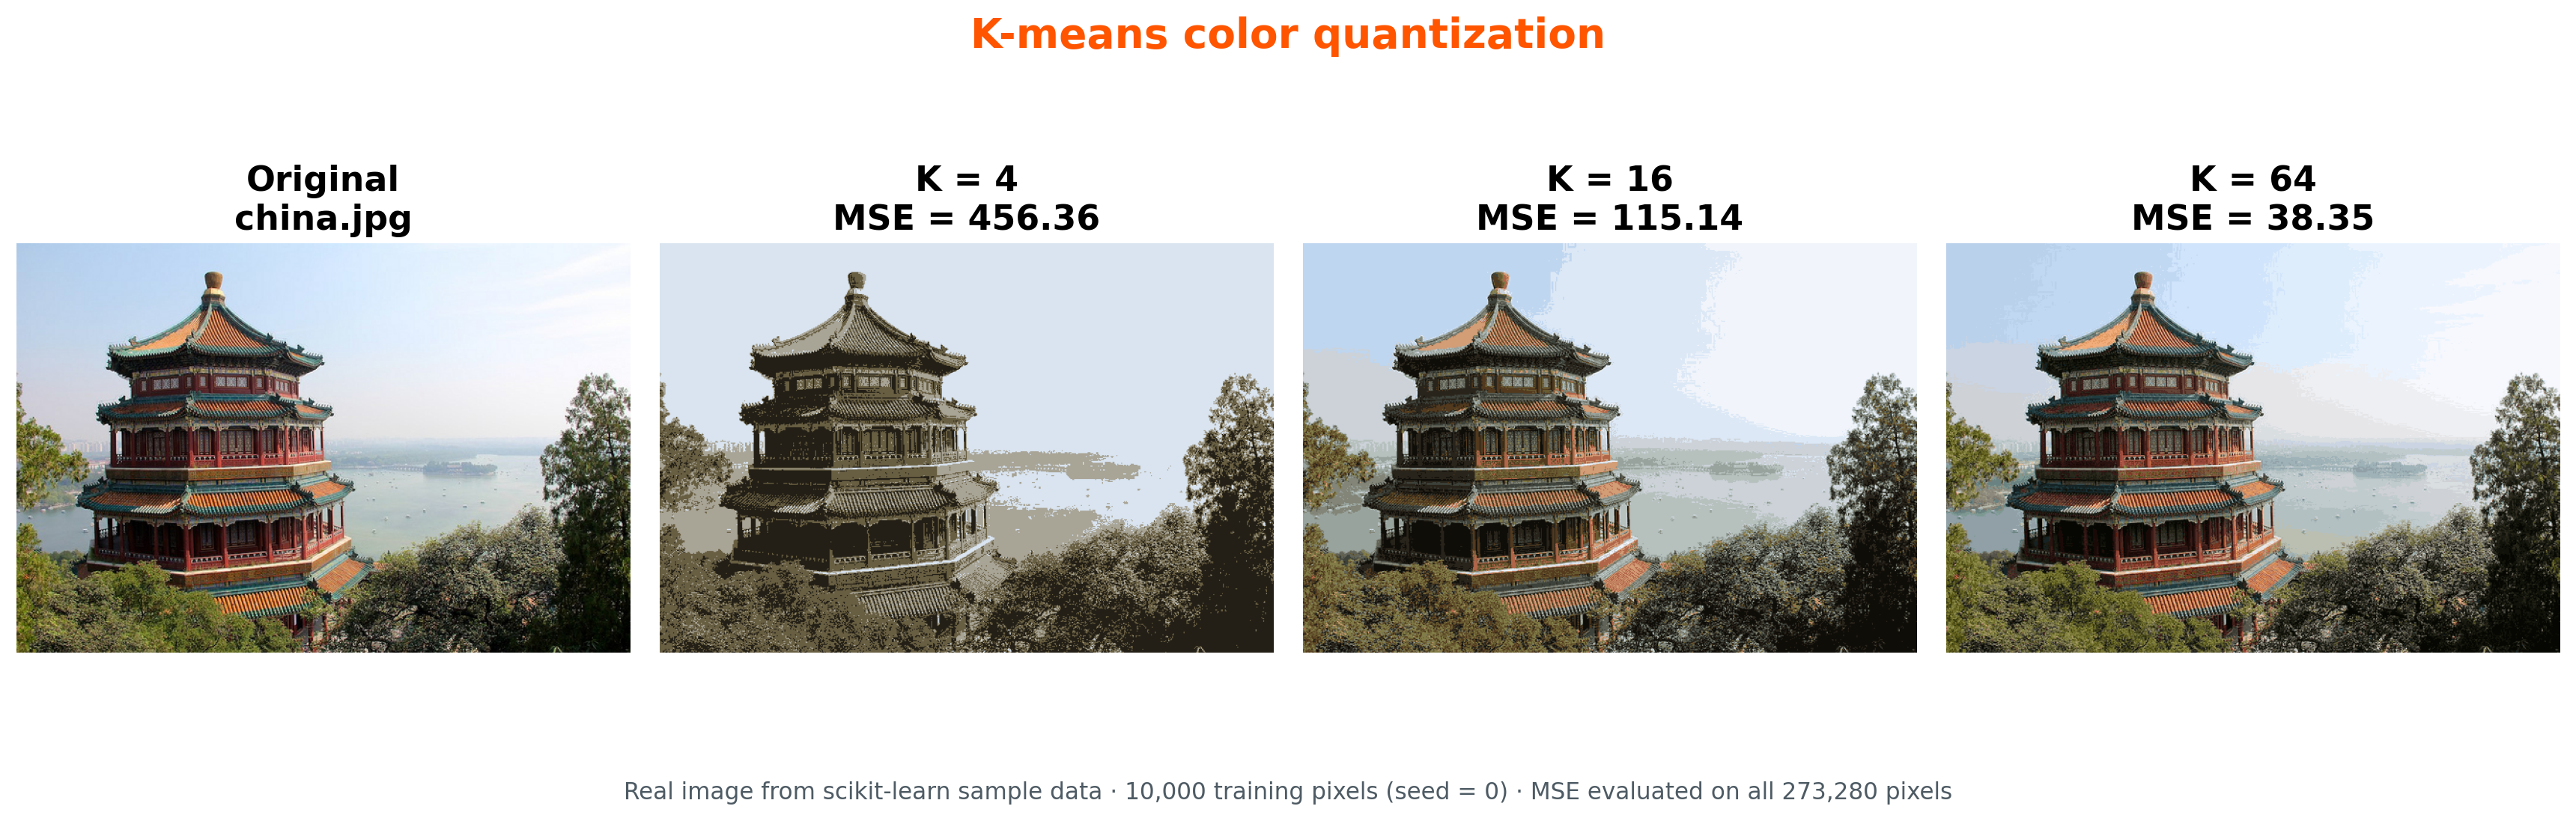
\includegraphics[width=.91\textwidth]{assets/motivation/kmeans_color_quantization.png}

  \vspace{.10cm}
  \scriptsize Each pixel is a point in RGB space; the cluster means form a compact color palette.

  \src{Image and example adapted from the \href{https://scikit-learn.org/stable/auto_examples/cluster/plot_color_quantization.html}{scikit-learn color quantization example}.}
\end{frame}

\begin{frame}{The Value of a Cluster Is Downstream}
  \begin{columns}[T,onlytextwidth]
    \column{.30\textwidth}
      \begin{tikzpicture}
        \node[softbox,text width=3.0cm] {\textbf{Explore}\\discover groups and inspect their profiles};
      \end{tikzpicture}
    \column{.30\textwidth}
      \begin{tikzpicture}
        \node[greenbox,text width=3.0cm] {\textbf{Summarize}\\replace many observations with prototypes};
      \end{tikzpicture}
    \column{.30\textwidth}
      \begin{tikzpicture}
        \node[orangebox,text width=3.0cm] {\textbf{Act}\\route, recommend, compress, or allocate};
      \end{tikzpicture}
  \end{columns}

  \vspace{.55cm}
  \begin{tikzpicture}
    \node[softbox,text width=10.2cm]
      {A partition is useful when it changes what we do next.};
  \end{tikzpicture}
\end{frame}

\begin{frame}{What Clustering Does Not Promise}
  \begin{columns}[T,onlytextwidth]
    \column{.46\textwidth}
      \textbf{It can provide}
      \begin{itemize}\spaceditems
        \item A reproducible partition under stated features and distance;
        \item A small set of prototypes or group profiles;
        \item A starting point for exploration or downstream modeling.
      \end{itemize}

    \column{.46\textwidth}
      \textbf{It does not provide automatically}
      \begin{itemize}\spaceditems
        \item Ground-truth categories;
        \item A unique answer independent of scaling or representation;
        \item A useful decision unless the groups support an action.
      \end{itemize}
  \end{columns}
\end{frame}
